\chapter{Introduction}


In the ever-expanding field of artificial intelligence, machine learning has achieved remarkable breakthroughs across a wide spectrum of applications. In recent years, the landscape of machine learning has undergone remarkable transformation, ushering in a new era of sophisticated models capable of tackling intricate challenges across diverse domains. These advancements have emerged as a direct consequence of the field's progress, allowing for the development of complex solutions that were previously unattainable. Amid this evolution, the classification of astronomical objects has emerged as a domain of paramount significance. The precise identification of stars, galaxies, and quasars assumes a pivotal role in advancing our comprehension of the universe's inner workings.

\section{Motive}
In the Research Methods module, the class was given an assignment of writing a research proposal as part of our learning objectives. Students were provided with a list of potential topics to help them find something they are interested in or might find interesting. Among the topics was Genetic Algorithms, which caught my attention since it was something I had not heard before. In order to learn more about this topic in depth, I decided to prepare a research proposal around the topic in order to get the opportunity to immerse myself in it more deeply. Based on my literature review, I found that genetic algorithms are extensively used to solve optimization problems. My interest was piqued by a paper which used genetic algorithms in order to fine-tune hyperparameters for machine learning models. Due to my background in astronomy, I was intrigued by the idea that genetic algorithms could be used to tune hyperparameters of models that are used in astronomy. The study would be extremely exciting because of its highly interdisciplinary nature. I find it fascinating when concepts and ideas give inspiration to concepts across different disciplines.

\section{Sloan Digital Sky Survey}
The Sloan Digital Sky Survey (SDSS) is an all-sky imaging survey that uses a large telescope measuring 2.5 meters in diameter to take pictures of the night sky. One of the best aspects of SDSS is the free public accessibility of the data. Very few research papers were published in the coinciding fields of computer science and astronomy which utilised the recently released new dataset - DR18 (Data Release 18). \cite{Wierzbiński} did a very similar study as this thesis but with a small dataset and the older version of data. I decided to build up on it and use a much larger dataset from the latest release and try to improve upon model performance by tuning the hyperparameters and/or validate the results of this paper.

\begin{figure}[H]
    \centering
    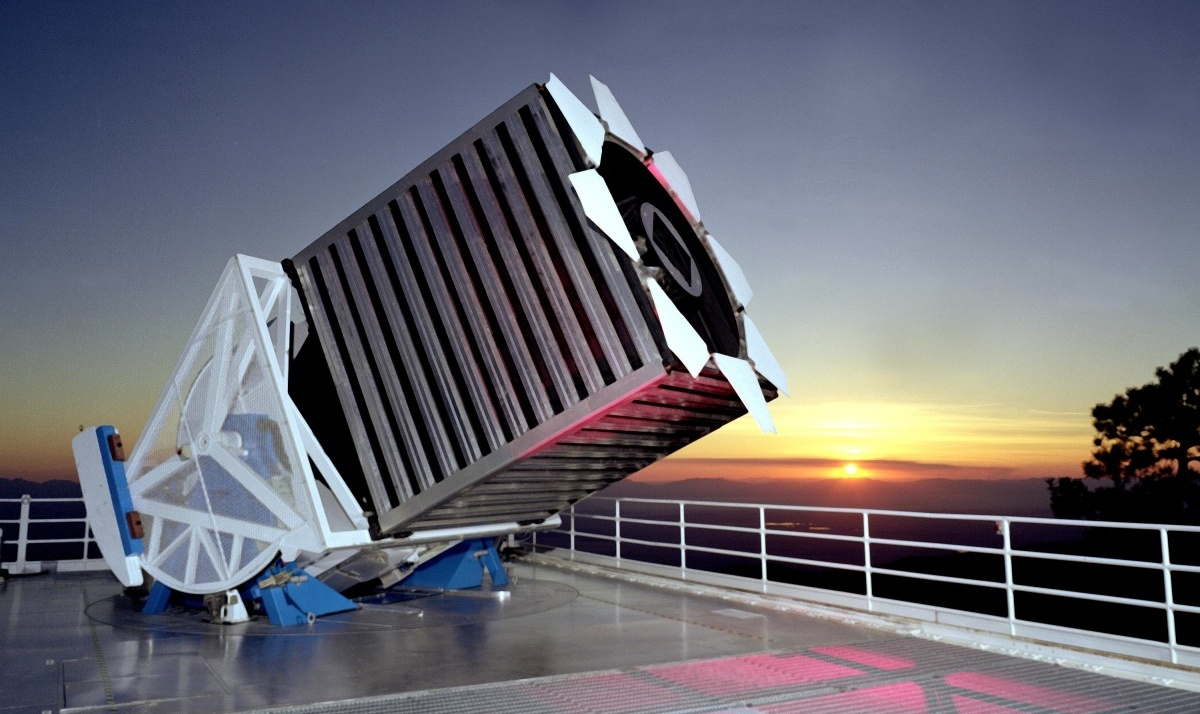
\includegraphics[scale=0.5]{images/sdss.jpeg}
    \caption{The SDSS 2.5 meter telescope \citep{sloanSloanDigital}}
    \label{fig:sdsstelescope}
\end{figure}

\section{Aim and objective}
Traditionally, the process of fine-tuning machine learning model hyperparameters has been a manual endeavor, involving human intervention to optimize performance. While this method has yielded notable outcomes, it bears the drawbacks of being labor-intensive, time-consuming, and susceptible to subjective biases. Genetic algorithms, underpinned by the evolutionary principles of natural selection, emerge as a class of optimization techniques that mimic genetic recombination and mutation. These algorithms iteratively refine and adapt solutions across multiple generations by encapsulating hyperparameters of machine learning models within a population of prospective solutions.

The research goal of this thesis is to use genetic algorithms to tune machine learning hyperparameters and to quantitatively evaluate the performance of machine learning models. Does genetic optimisation work effectively to tune hyperparameters and improve model performance? Does implementation of genetic algorithm incurr high computational costs? This will help us decide if it is feasible to use this algorithm or not. These are the research questions that I aim to answer.

\section{Structure of this document}

I have structured the document in a way which will help the reader comprehensively explore the research undertaken. The next chapter is indepth literature review which summarises the current knowledge about all the concepts, tools and technolgies relevant to the thesis. It commences by delving into the SDSS's role in the realm of astronomical observation, followed by a comprehensive survey of previous works in this domain. The chapter further delves into machine learning, offering detailed insights into various techniques such as Random Forest Classifier, Gradient Boosting Classifier, Logistic Regression, Support Vector Machines, Cross Validation, Overfitting, Underfitting, and Machine Learning Metrics. 

This is followed by chapter titled Methodology which gives a roadmap of research method that was implemented. It initiates with the intricacies of data collection, followed by a thorough examination of preprocessing and feature selection techniques. The establishment of baseline performance serves as a pivotal point before transitioning into the core of the methodology—the implementation of Genetic Algorithms. The chapter concludes by outlining the evaluation process and criteria used to gauge the results.

Observations and findings chapter begins with an in-depth exploration of Exploratory Data Analysis (EDA), uncovering insights from the data. It then systematically dissects the performance of each model employed, the Random Forest Classifier, Gradient Boost Classifier, and Logistic Regression. 

Finally, Chapter 5 draws conclusions, it summarizes the findings, creating a coherent narrative that addresses the research objectives. The conclusions offer a succinct summary of the research's contributions and implications, while also acknowledging areas of potential expansion and further exploration.

